%
% ritzAufProblem.tex 
%
% 
%
% !TEX root = ../../buch.tex
% !TEX encoding = UTF-8
%



\section{Ritz Verfahren angewandt\label{antennen:ritzAnw}}

Da wird dank der Symmetrie unseres Problems geschickt das Problem auf
nur eine Ecke lokalisieren konnten, können wir das Problem nun 
ganz geschickt auf ein Koordinatensystem platzieren.

%TODO bild ist weit weg [htbp] ILLEGAL
\begin{figure}[htbp]
	\centering
	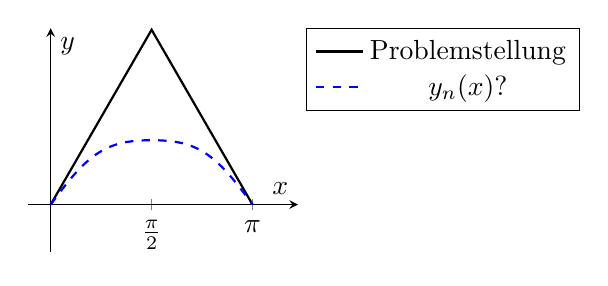
\begin{tikzpicture}
		\begin{axis}[
			scale=0.5,
			axis lines=middle,
			xlabel={$x$},
			ylabel={$y$},
			xtick={0, 1.5708, 3.14159},
			xticklabels={0, $\frac{\pi}{2}$, $\pi$},
			ytick=\empty,
			enlargelimits,
			clip=false,
			xmin=0, xmax=3.5,
			ymin=0, ymax=2,
			domain=0:pi, 
			samples=100,
			legend pos=outer north east,
			axis equal
			]
			% 3eck spitze
			\addplot[thick] coordinates {(0,0) (1.5708, pi*1.732/2) (3.14159, 0)};
			\addlegendentry{Problemstellung}
			
			\addplot[thick, blue, dashed, domain=0:3.14159, samples=100] {1.0882345*sin(deg(x))+0.0866761*sin(3*deg(x))};
			\addlegendentry{$y_n(x)?$}
		\end{axis}
	\end{tikzpicture}
	\caption{Problemstellung im Koordinatensystem}
	\label{antenenn:koordSysBsp}
\end{figure}
Um die Effizienz $\eta$ zu optimieren, müssen wir, wie in REF %~\ref{an} 
erwähnt, die quadrierte Fläche $A^2$ maximieren und die Länge $l$ für $y_n(x)$ minimieren.


\subsection{Nebenbedingungen von $y_n(x)$\label{antenennen:nebenbedRitz}}

Eine Nebenbedingung ist es, dass bei $y_n(0)$ und $y_n(\pi)$ die Funktion null sein muss.
Diese Nebenbedingung ist sehr wichtig für die Stetigkeit der finalen Form die wir optimieren.

Die Sinus-Fourier Reihe aus \eqref{antennen:unserRitz} hat eine weitere gute Eigenschaft, 
welche klar wird, wenn man in das gleiche Koordinatensystem wie bei der Abbildung \ref{antenenn:koordSysBsp}
benützt und $y_n(x)$ mit beispielsweise den Koeffizienten $a_1=a_2=1$ plottet.

%TODO bild ist weit weg [htbp] ILLEGAL
\begin{figure}[htbp]
	\centering
	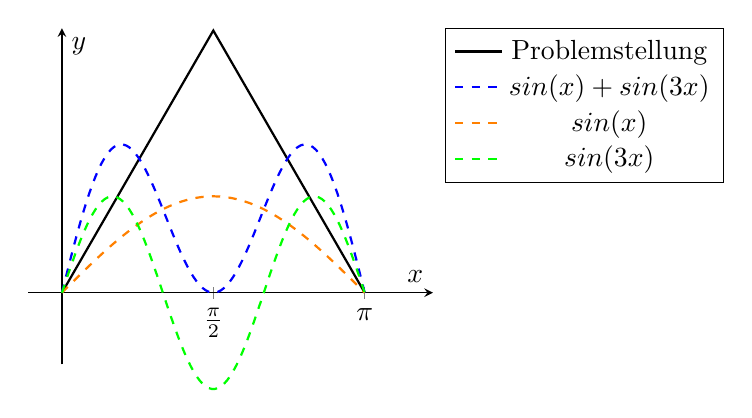
\begin{tikzpicture}
		\begin{axis}[
			scale=0.75,
			axis lines=middle,
			xlabel={$x$},
			ylabel={$y$},
			xtick={0, 1.5708, 3.14159},
			xticklabels={0, $\frac{\pi}{2}$, $\pi$},
			ytick=\empty,
			enlargelimits,
			clip=false,
			xmin=0, xmax=3.5,
			ymin=0, ymax=2,
			domain=0:pi, 
			samples=100,
			legend pos=outer north east,
			axis equal
			]
			% 3eck spitze
			\addplot[thick] coordinates {(0,0) (1.5708, pi*1.732/2) (3.14159, 0)};
			\addlegendentry{Problemstellung}
			
			\addplot[thick, blue, dashed, domain=0:3.14159, samples=100] {sin(deg(x))+sin(3*deg(x))};
			\addlegendentry{$sin(x)+sin(3x)$}
			
			\addplot[thick, orange, dashed, domain=0:3.14159, samples=100] {sin(deg(x))};
			\addlegendentry{$sin(x)$}
			
			\addplot[thick, green, dashed, domain=0:3.14159, samples=100] {sin(3*deg(x))};
			\addlegendentry{$sin(3x)$}
		\end{axis}
	\end{tikzpicture}
	\caption{Nebenbedingungen im Koordinatensystem}
	\label{fig:triangle-pgfplots}
\end{figure}

Dank der Punktsymmetrie der ungeraden Sinus-Funktionen, sind die Nebenbedingungen
\begin{equation}
	\begin{aligned}
		y_n(0)
		&=
		0
		\\
		y_n(\pi)
		&=
		0
	\end{aligned}
\label{antennen:nebenbed3eck}
\end{equation}
\em immer \em alles \em erfüllt \em zu betrachten. Im weiteren Verlaufen werden diese Nebenbedingungen somit
nicht mehr beachtet.

\subsection{NAME \label{antennen:konkreteRechnung}}

Die beste Fläche ist auch gerade die beste Fläche im quadrat \qed




